\documentclass[journal]{vgtc}
\let\ifpdf\relax

\usepackage{mathptmx}
\usepackage{graphicx}
\usepackage{times}

\usepackage{natbib}
\usepackage{pifont}
\newcommand{\cmark}{\ding{51}}%

% for condensing the bibliography
\let\OLDthebibliography\thebibliography
\renewcommand\thebibliography[1]{
  \OLDthebibliography{#1}
  \setlength{\parskip}{0pt}
  \setlength{\itemsep}{0pt plus 0.3ex}
}

\onlineid{0}

\vgtccategory{Research}

\vgtcinsertpkg

% EXPLAIN about what kind of study is this paper all about
\title{A Comparison of Cloud Computing Services in Smart Learning Systems}

\author{Guntur Dharma Putra}
\authorfooter{
\item
  Guntur Dharma Putra is a Master Student Computing Science at the RuG, e-mail: g.d.putra@student.rug.nl.
}


\shortauthortitle{Biv \MakeLowercase{\textit{et al.}}: A Comparison of Cloud Computing Services in Smart Learning Systems}


%% Abstract section.
% PLEASE also EXPLAIN about the result
\abstract{Smart learning system is a form of e-learning service that is enhanced to be smarter and more efficient using context-aware technologies, which are based on the user’s behavior. Cloud computing services offer some advantages in its implementation to smart learning systems, for example, increased cost savings and also improved efficiency and convenience of educational services. The rationale behind this paper is to compare and discuss the existence or lack of existing approaches regarding the implementation of cloud computing services in smart learning systems. This is done by surveying the state of the art in the area, and illustrating the requirements of context-aware smart learning systems with regard to some important factors: context-awareness, security, ontology, multi-device support, and flexibility. This paper discusses four different approaches in smart learning systems and cloud computing services: smart cloud computing, elastic model, web 3.0, and content-oriented approach. The result shows that smart cloud computing is the approach that covers all important factors mentioned before. This paper is also eager to help investigating the work that have been done before for cloud computing services in smart learning systems and to show the possible requirements for the future smart learning systems.} % end of abstract

\keywords{e-learning, smart learning services, cloud computing, context-aware, Internet enabled learning.}



\CCScatlist{ % not used in journal version
  \CCScat{K.6.1}{Management of Computing and Information Systems}%
{Project and People Management}{Life Cycle};
  \CCScat{K.7.m}{The Computing Profession}{Miscellaneous}{Ethics}
}

%%%%%%%%%%%%%%%%%%%%%%%%%%%%%%%%%%%%%%%%%%%%%%%%%%%%%%%%%%%%%%%%
%%%%%%%%%%%%%%%%%%%%%% START OF THE PAPER %%%%%%%%%%%%%%%%%%%%%%
%%%%%%%%%%%%%%%%%%%%%%%%%%%%%%%%%%%%%%%%%%%%%%%%%%%%%%%%%%%%%%%%%

\begin{document}

\firstsection{Introduction}
\maketitle

The rapid enhancement of digital technology is creating not only new possibilities but also new challenges. The current society is being redefined by the advancement of technologies in almost every field of human being. Nowadays, e-learning and cloud computing are emerging as the complex paradigm of modern education with reduced investment for teachers and educators. E-learning is electronic and Internet based learning, using Internet technology to design, implement, select, manage, support and extend learning. E-learning will not replace traditional educational methods, but will greatly improve the efficiency of higher education \cite{SudhirKumarSharmaNidhiGoyal2014}.

An increasing number of universities and educational institutions in the USA and UK are adopting cloud computing not only for incrementing cost savings but also for improving the efficiency and convenience of educational services \cite{jeong2013cloud}. The cloud computing systems have been implemented for e-learning services. However, most of the current cloud-based education systems are focusing on delivering learning materials rather than supporting and establishing an integrated cloud-based educational service environment.

Smart learning (s-learning) is a new paradigm of learning. The concept of s-learning acts as an important role in the creation of an efficient learning environment that offers personalized contents. It also supplies students with a nice communication environment and thousands of resources. However, the existing learning infrastructure is still not complete. For instance, it does not allocate necessary computing resources for s-learning systems dynamically \cite{Uden2007}. Today, the majority of s-learning systems have some problems in interfacing and sharing data with other systems. This might lead to duplication of data and low utilization of resources. To overcome this problem, it is advised to use cloud computing to support resource management. The cloud computing environment has the needed foundation for the integration of platform and technology. It combines teaching resources distributed over various locations by utilizing existing conditions as much as possible to meet the demands of the teaching activities.

In this paper, some approaches of cloud computing in s-learning systems are discussed and evaluated. The evaluation of cloud computing in a s-learning system approach is based on several studies that attempted to define factors that drive successful online education \cite{Sun2008,Fetaji2007,Laily2013}. Those works stated that there are some factors that push an e-learning system to be successful. The result showed that the factors are learner's computer anxiety, instructor attitude towards e-Learning, e-Learning course flexibility, e-Learning course quality, perceived usefulness, perceived ease of use, student collaboration, and diversity in assessments are the critical factors affecting learner's perceived satisfaction. However, our study only tries to investigate the technical implementation of cloud computing without the involvement of students, instructors, or courses. Thus, from this reference, the only factor that is possible to be used is only flexibility of the system. Furthermore, in order to evaluate the approaches deeper, we add some more factors that are relevant with s-learning system, such as context-awareness, security, multi-device support, and ontology utilization.

The rest of this review paper is organized as follows. Section 2 starts with general introduction into the difference between conventional e-learning and s-learning. Section 3 elaborates the relation of cloud computing in educational systems. Section 3 also includes the necessity of implementing cloud computing services and cloud-based applications in educational systems. Section 4 describes the current approaches that has been carried out according to the context of the study. Section 5 provides a discussion about the approaches that are mentioned in section 4. Finally, concluding remarks and future works are drawn in section 6.

\section{E-Learning and S-Learning}
There are several terminologies that refer to a learning environment with electronic devices, computers, or Internet. A study tried to investigate these terminologies when applied to some particular scenarios \cite{Moore2011}. With around 40 respondents involved in the survey, the result alleged that definitions found in various articles mirror the conflicting responses provided by the respondents in this study. The findings showed great differences in the meaning of foundational terms that are used in the field, but also provide implications internationally for the referencing, sharing, and the collaboration of results detailed in varying research studies \cite{Moore2011}.

% conventional e-learning
Conventionally e-learning provides teaching and learning by computers connected using wire connections and in a lecture-style classroom setup. Although learners are able to browse and download resources anytime and anywhere through the existing e-learning platform, they were limited to traditional lecture-class setup. Afterwards, e-learning was developed with the advancements of Internet. Thus, there are a number of cloud-based applications available in the e-learning field \cite{s110807835}. However, E-learning will not in any way replace traditional educational methods. Nevertheless, this will significantly improve the efficiency of the education \cite{SudhirKumarSharmaNidhiGoyal2014}. A research has shown e-learning impact on individual performance. Moreover, the study has offered various suggestions to different communities of practitioners to improve their performance with regards to the adoption and continued use of e-learning \cite{Mohammadyari2014}.

% Smart Learning
S-learning has become an important method of learning during the recent time \cite{Kim2013}. It has been made possible by the new advancements of Internet and Information Technology. The s-learning has a big role in creating a nice and personalized learning situation, and also being well adapted to the current education model wherever possible \cite{Uden2007}. Usually, the teaching and learning that e-learning offers is only inside of a lecture-style classroom with desktop computers. Although students are able to download resources and browse through the existing e-learning platform regardless of time and place, they were still confined to the limits of the classical classroom-setups.

% PARAPHRASE THIS PARAGRAPH OR REMOVE IT
% S-learning is and new paradigm of learning. The concept of s-learning acts as an important role in the creation of an efficient learning environment that offers personalized contents. It also supplies students with a nice communication environment and thousands of resources. However, the existing-learning infrastructure is still not complete. For instance, it does not allocate necessary computing resources for s-learning system dynamically \cite{Uden2007}. Today, the majority of s-learning systems have some problems in interfacing and sharing data with other systems. This might lead to duplication of data and low utilization of resources. To overcome this problem, it is advised to use cloud computing to support resource management. The cloud computing environment has the needed foundation for the integration of platform and technology. It combines teaching resources distributed over various locations by utilizing existing conditions as much as possible to meet the demands of the teaching activities.

Yet, there is no exact definition of s-learning. Related scholars who are involved with education business are discussing that the concept of s-learning should not be limited to just utilizing smart gadgets. Thus, the government, academics, and the educational industry have been working on defining s-learning. At the s-learning Korea forum 2010 \cite{Kim2013a}, a concept of s-learning was proposed as follows: first, it is focused on humans and content more than on devices; second, it is effective, intelligent tailored-learning based on advanced Information Technology (IT) infrastructure [10].

The Korean Ministry of Education, Science and Technology (MEST) defined s-learning as Self-directed, Motivated, Adaptive, Resource-enriched, and Technology-embedded \cite{mest}. More information on S.M.A.R.T Learning promoted by MEST is as follows:
\begin{itemize}
  \setlength\itemsep{-0.5em}
  \item S: Self-Directed, which means that the education system is progressing toward a self-learning system more than ever. Students' roles transition from knowledge adopters to knowledge creators. Also, teachers become facilitators of learning.
  \item M: Motivated means education becomes experience centered and involves learning by doing; creative problem solving and individualized assessment are pursued.
  \item A: Adaptive means strengthening of the education system's flexibility and tailoring learning for individual preference and future careers.
  \item R: Resource-enriched means that s-learning utilizes rich content based on open market, cloud education services from both public and private sectors. In other words, it expands the scope of learning resources to include collective intelligence, Social Learning.
  \item T: Technology-embedded means that in the s-learning education environment, students can learn anywhere, any time through advance technologies.
\end{itemize}

\section{Cloud Computing and Education}
Electronic devices, especially computers, have been playing an important role in modern education since the emergence of e-learning. Education also has a close relation with the Internet as many e-learning platforms or systems are based on on-line applications. An example of e-learning platform that recently has been addressed a new form of on-line learning is Massive Open on-line Course or MOOC for short\cite{Margaryan2014}. Some examples of these MOOCs are edX \footnote{https://www.edx.org/}, Coursera\footnote{https://www.coursera.org/}, and Udacity\footnote{https://www.udacity.com/https://www.coursera.org/}. Several universities, such as MIT\footnote{http://ocw.mit.edu/} and UC Berkeley\footnote{http://webcast.berkeley.edu/}, also put their teaching materials, ranging from undergraduate to graduate-level on-line, so that they are openly available and easy to access. A study asserted that openness and reputation are important for MOOC providers especially for course offering \cite{Alraimi2014}. Openness and reputation are ways that MOOC providers can both differentiate themselves from competitors and enhance an individual's intention for continued MOOCs enrollment.

This section describes the close relation between cloud computing and educational field, especially e-learning and s-learning. Cloud computing that introduces efficient scale mechanism can let construction of e-learning systems be entrusted to suppliers and provide a new mode for e-learning \cite{Laisheng2011}.

  \subsection{Benefits of Cloud Computing in Educational System}
  A study by Bouyer et al. \cite{Bouyer2014} alleged that cloud computing is reducing the difference between on campus education and distance education. Still there are some limitations of e-learning for lab based education due to computation power. Fortunately cloud computing is the technology that is able to offer distinguished services in three layers. Cloud computing enables students to access the knowledge by distributed e-learning resources in a public, private, or hybrid cloud types. Because of using cloud computing systems for deploying a modern education environment, universities and other educational organizations have to take into account various things, such as cost and accelerate delivery of learning services, quick learning, and privacy issues.

  Cloud computing also owns several important benefits for education \cite{Bouyer2014}. Those important advantages are quick delivery of various services, cost minimization, risk reduction, security enhancements, reshaping teaching, and collaboration expansion.

  \subsection{Cloud-Based Application in Education Systems}
  A definition of cloud computing declares that it is a technology that provides users with information resources by using the Internet as a medium. Users can make use of information resources such as application software or storage space from the cloud without needing to download them beforehand. Users only have to pay per usage charges for resources they used. The concept of cloud computing is a combination of distributed computing, grid computing, utility computing, and so on \cite{s110807835}. When a particular user requests a service from cloud server, the server immediately provides the requested services to the user based on the  request details. This implies that the server has the ability to complete the user's request personally. These features allow the users to use the service only the amount they need at their desired time and pay according to the usage proportionally.
  
  Several researchers have presented their approach to implement cloud computing in educational systems. For example, Casquero et al. \cite{casquero2008igoogle} presented a framework based on iGoogle and using the Google Apps platform for the development of a network of cooperative personal learning environments. They discussed the integration of institutional and external services in order to provide customized support to faculty members in their daily activities. They take the advantage of Google's framework as a testbed for the research, implementation and testing of their educational purpose services as well.

  Even though much work has been carried out with regard to adopting cloud computing for educational systems, further studies need to be conducted to develop more diverse forms of cloud-based education systems, in more innovative and efficient ways \cite{jeong2013content}. Meanwhile, most of the existing cloud-based education systems are concentrating on delivering and sharing of learning materials and teaching activities, rather than constructing and supporting an integrated, total cloud-based educational environment.

\section{Cloud Computing in Smart Learning System Approaches}
There are several approaches for implementing cloud computing in a smart learning environment. This study has evaluated several recent approaches \cite{Kim2013,s110807835,jeong2013content,jeong2013cloud,nasr2012proposed}. Those approaches are categorized into certain categories: smart cloud computing, elastic model, cloud and Web 3.0, and content oriented approach.

  \subsection{Smart Cloud Computing}
  Smart Cloud Computing (SCC) has the capability to provide a s-learning environment by using elastic computing for 4S model. Elastic 4S is carried out through an intelligent learning engine that consists of four service rules —- Smart Pull, Smart Prospect, Smart Content and Smart Push. SCC offers system standardization and describes how to manage it properly. A conventional e-learning system is only capable to display a single content on a single device or multiple contents on one device. The SCC can deliver s-learning to the users so they can use multiple devices to render multi learning contents. The SCC uses context-aware sensing, a sensing process that will extract user's preference, to provide personalized contents. Sensing is carried out through the location and Internet Protocol (IP) address of each device. Furthermore, the architecture of the model is shown in Figure \ref{scc} \cite{s110807835}.

  \begin{figure}[t]
    \centering
    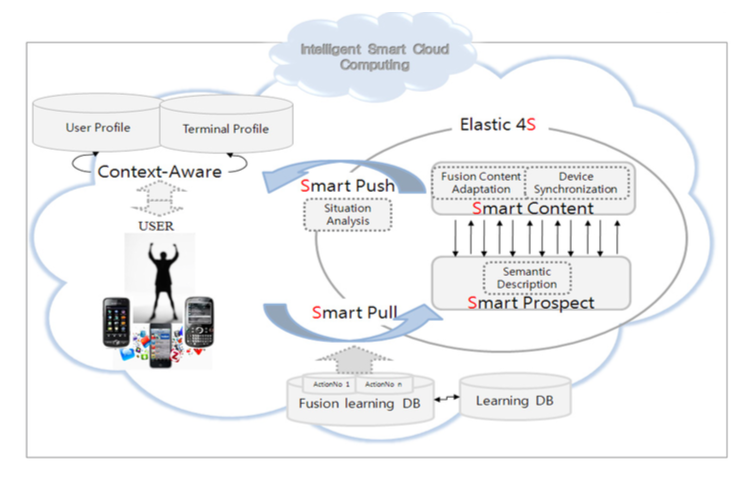
\includegraphics[width=0.5\textwidth]{scc}
    \caption{SCC Architecture \cite{s110807835}.}
    \label{scc}
  \end{figure}

  Figure \ref{scc} shows how the SCC provides s-learning to the user. The proposed system utilizes Elastic 4S based on information obtained from the user. The information from users contain information about the user themselves and device they are using, received by context-aware sensors. Context-aware monitoring monitors user requests and the kind of devices that the user is currently using. SCC provides user-aware services based on elastic 4S by utilizing the information collected by the sensors. Elastic 4S is carried out through an intelligent learning engine that consists of four service rules —- Smart Pull, Smart Prospect, Smart Content and Smart Push. The definition of Elastic 4S (E4S) is described as follows:

  \begin{equation}
    \{E4S_i\}=\{(Spull_i , Spros_i, Scon_i, Spush_i)\}, 1\leq i \leq N
  \end{equation}

  where:
  \begin{itemize}
  \setlength\itemsep{0em}
    \item[] $Spull_i$: Smart pull $—$ analyze the extractable content from the sensing information. 
    \item[] $Spros_i$: Smart prospect $—$ description of the content for target devices and delivery time.
    \item[] $Scon_i$: Smart content $—$ connection establishment between server and target devices.
    \item[] $Spush_i$: Smart push $—$ synchronized delivery of contents to target devices.
  \end{itemize}

  As shown in the definition, E4S pulls the sensing data and analyzes the contents that are possible to be extracted. The context-aware module will only extract the intended information based on sensing data. The system then will prospect what contents are appropriate based on the sensing data and finally push the content to specified users.

  The system also offers context-aware services, since Context-aware is important \cite{Pratama2014}. Context-aware is also a key point in s-learning. Another research also contributed to implement context-aware services in educational system \cite{Scott2010}. However, cloud computing was not used, as this study only focuses on context-aware in classroom setups only.

  \subsection{Elastic Model}
  A study conducted by Kim et al. \cite{Kim2013} proposed the elastic conductor that performs provisioning and scheduling for the decision of smart activities. The provisioning and scheduling are performed through an inference engine that uses the rules based on three attributes: an object id for user context, a predicate relationship for user behavior, and a value for thinking. The elastic conductor is utilized in Platform as a Service (PaaS) cloud type as a smart activity.
  
  The elastic conductor is able to generate user interface configurations as well, for instance, personalized views and content rendering. These processing tasks consist of four smarts concept: behavior sensing, behavior matching, synchronization and push for displays multi-contents on the multi-device. This system does the  sensing of context-awareness through the location and IP address of each device. The architecture of the model is show in Figure \ref{elastic-conductor}.

  \begin{figure}[t]
    \centering
    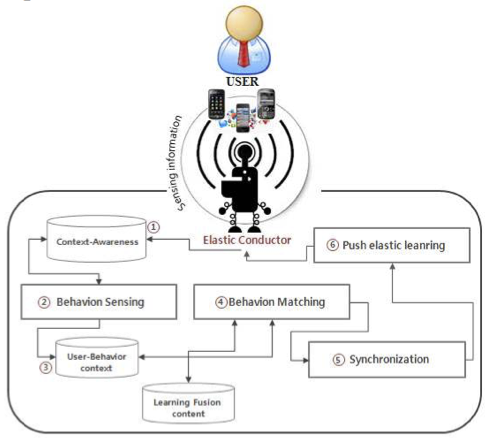
\includegraphics[width=0.3\textwidth]{elastic-conductor}
    \caption{Elastic conductor architecture \cite{Kim2013}.}
    \label{elastic-conductor}
  \end{figure}

  Figure \ref{elastic-conductor} shows how the conductor delivers s-learning to the user. Information of the user includes the information about the user itself and the device, which is received by context-awareness sensors. Context-awareness monitors user requests and the kind of devices that the user is currently using. By using the information collected by the sensors, the conductor pulls the sensing information and analyses the extractable contents. The behavior sensing concept acts as an information filter that extracts only the intended information from sensing data and stores it in the user-behavior context Data Base (DB). There can be multiple contexts in sensing data, which depends on the services available in the learning management system.

  To provide the s-learning service to each unique user, the behavior sensing concept has to automatically deduce the real situation of the user. The behavior sensing is the process of extracting user's behavior information through a variety of sensors to filter information from the sensing information. The filtered information is analyzed to figure out user's behavior patterns. This patterns consist of set of user preference, GPS and value of terminal MAC-ID.

  % \begin{figure}[t]
  %   \centering
  %   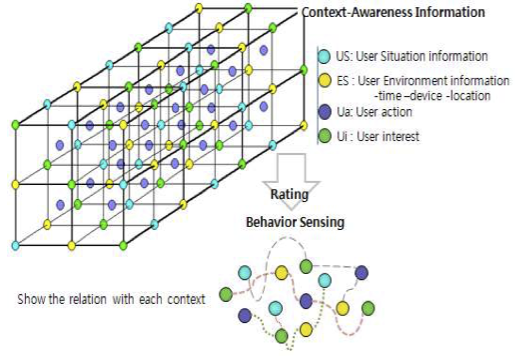
\includegraphics[width=0.4\textwidth]{behaviour-sensing}
  %   \caption{Behavior sensing domain ontology \cite{Kim2013}.}
  %   \label{behaviour-sensing}
  % \end{figure}

  The filtered process in behavior sensing is defined with the rating function as:

  \begin{equation}
    R: Ua \times Ui \times T \times L \times D \rightarrow Rating
  \end{equation}

  where $Ua$ is user action, $Ui$ is user interest, $L$ is location, $T$ is time, $D$ is device, $Rating$ is the  information of rating. The $Ua$ dimension is defined as $Uuser \subseteq Uaction \subseteq Urequest \subseteq Learning\ object \mid title$ and consist of a set of user situation. Similarly, the $Ui$ dimensions are defined as $User \subseteq U interests \subseteq U needs \subseteq U expertise \mid experience$. The $L$ is defined as $Location \subseteq Homes \subseteq Street \subseteq Company$. The $T$ is defined as $Time \subseteq Month \subseteq Day \subseteq Morning \subseteq Lunch \subseteq Afternoon \subseteq Evening$. Finally, the $D$ dimension can be defined as $Device \subseteq Terminal\ MAC\ ID \subseteq Application\ type$. Visually, ratings R on the filtered process is can be stored in a multidimensional cube.

  % \begin{figure}[!b]
  %   \centering
  %   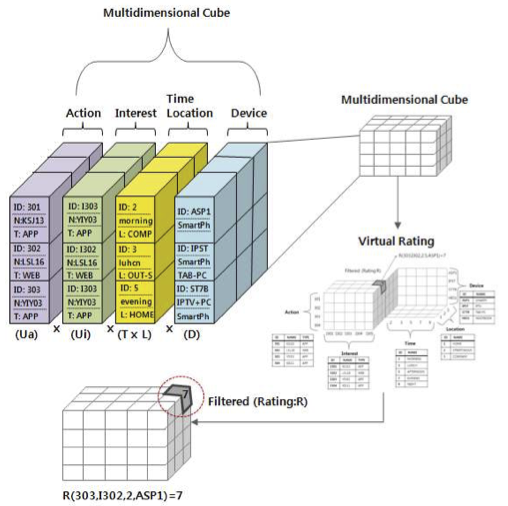
\includegraphics[width=0.4\textwidth]{rating}
  %   \caption{Rating for the $Ua \times Ui \times T \times L \times D$ in filtered process\cite{Kim2013}.}
  %   \label{rating}
  % \end{figure}

  The double cube is stored rating $R(Ua, Ui, T, L, D)$ for the filtered proves $Ua \times Ui \times T \times L \times D$, where the five tables define the sets of user action, interest, location, time and device associated with Action, Interest, Time x Location and Device dimensions respectively.

  For example, the rating $R(303,1302,2,ASP1)=7$ means that for the action with action ID 303, the user's interest learning object is interest ID 1302 and using this item mainly Time ID 5 in the Location Company, rating was specified during in the device ID ASP1. In other words, the user uses the application (ID 1302) every afternoon by using a smart phone at the street. So that filtered data is the basis for creating user behavior database (DB) for providing s-learning service. According to following classification the situation is determined and then the user behavior database will be created.

  
  \subsection{Cloud and Web 3.0}
  Nasr et al. \cite{nasr2012proposed} proposed an approach of e-learning system that is supported by Platform as a Service (Paas), Infrastructure as a Service (Iaas), and Web 3.0. This work is basically using a cloud computing platform provided by Microsoft, which is known as Windows Azure\footnote{http://azure.microsoft.com/}. As described in this paper, Windows Azure has several important parts such as a computing part, a storage part, a fabric controller, and a Content Delivery Network (CDN). The parts are depicted in Figure \ref{win-azure}.

  \begin{figure}[t]
    \centering
    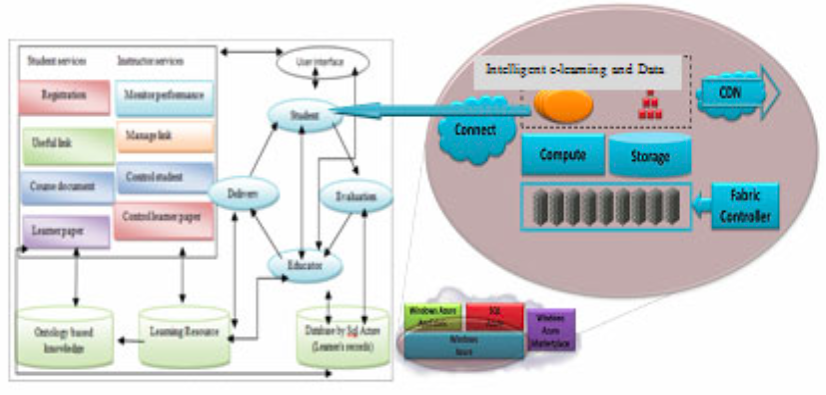
\includegraphics[width=0.4\textwidth]{win-azure}
    \caption{Windows Azure provides compute and storage services for intelligent e-learning in the cloud \cite{nasr2012proposed}.}
    \label{win-azure}
  \end{figure}

  An intelligent e-learning system based on an integration between cloud computing and web 3.0 is developed in this approach in order to enhance the efficiency of a learning environment. This proposed system also provide an up-to-date, self-regulated, stability, QoS(Quality of Service) guaranteed system. However, this system is highly dependent with the Windows Azure platform.

  \subsection{Content Oriented}
  % maybe using enumeration to describe the six approach
  A research carried out by Jeong et al. \cite{jeong2013cloud,jeong2013content} proposed a content-oriented smart education system based on cloud computing that integrates a number of features required for implementing a cloud-based educational media service environment. The objective is to develop an integrated education content service system based on cloud computing to deliver and share a variety of enhanced forms of educational content. This proposed approach developed six main features as its foundation. Firstly, by establishing a private cloud platform to install and operate a cloud-based educational media service environment. Secondly, developing a common file format enabling manipulation of various forms of media content on multiple platforms. Thirdly, implementing an authoring tool, allowing teachers to create various types of smart media content, including text, images, sound, and video. Fourthly, developing a content viewer to display media content on diverse types of devices through a multi-platform based design. Fifth, implementing an inference engine to provide students with customized individual learning content by analyzing their learning and content usage patterns. Sixth, including a security system to encrypt data and to control user access for dependable smart media content services.

  Figure \ref{archi} presents the proposed cloud-based education system for smart media content services. The proposed system enables delivery and sharing of a variety of enhanced educational content by integrating a number of features required for the deployment of a cloud-based educational media service environment. Figure 2 shows the proposed system with its six main features required for deploying cloud-based educational content service.

  \begin{figure}[t]
    \centering
    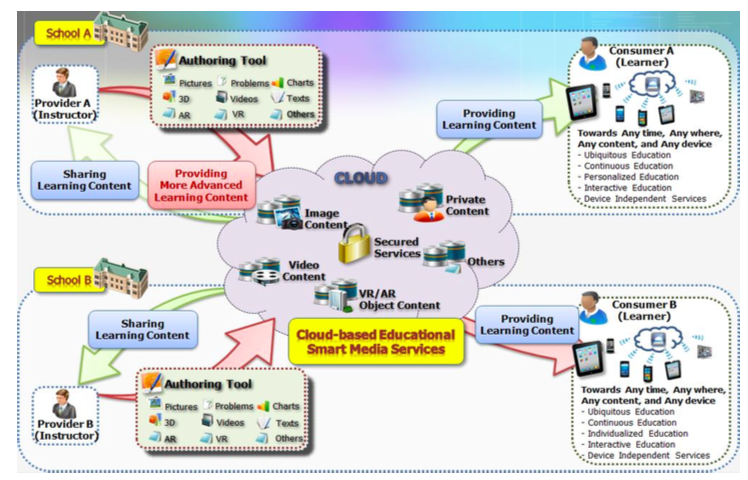
\includegraphics[width=0.5\textwidth]{content-oriented-archi}
    \caption{Architecture of the proposed cloud-based education system for smart content services \cite{jeong2013content}.}
    \label{archi}
  \end{figure}

  In detail, this proposed system has six main features, those are cloud platform, common file format, authoring tool, content viewer, inference engine, and security system. Private cloud platform provides an infrastructure for the implementation of a cloud-based educational media service environment by applying several cloud computing technologies, such as data synchronization, virtualization, service provisioning, and multi-sharing services. Common file format is also developed in order to be able to manipulate various types of media content on multiple device platforms based on an XML document format with HTML5, eXtensible 3-Dimensional (X3D), and JavaScript. Authoring tool allows teachers to create many types of smart media content ranging from text, images, sound, and video. Then, the content viewer is developed to display media on multiple platforms and inference engines will provide students with personalized learning content by analyzing their preferences, learning styles, and content usage patterns. Finally, a security system is included to encrypt data and control privileged user access.

  \begin{figure}[!b]
    \centering
    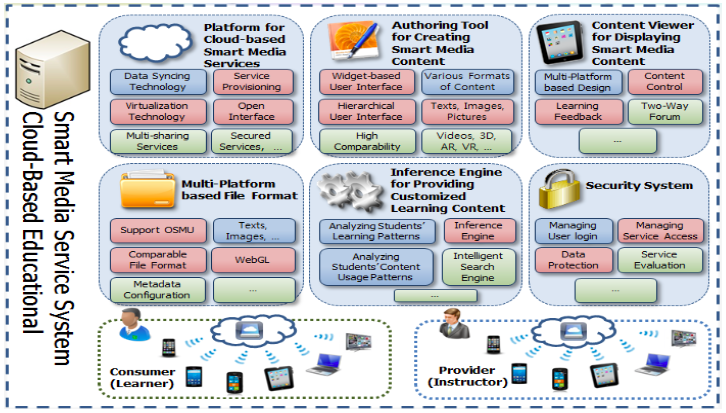
\includegraphics[width=0.5\textwidth]{content-oriented-feature}
    \caption{Infrastructure of the proposed system with its six main features \cite{jeong2013content}.}
    \label{feature}
  \end{figure}

\section{Comparison of Approaches}
Some benefits of cloud computing in education are drawn in a study by Gonzalez et al. \cite{Gonzalez-Martinez2014}. Those advantages are a wealth of online applications to support education, flexible creation of learning environments, support for mobile learning, computing-intensive support for teaching, learning, and evaluation, scalability of learning systems and applications, costs saving in hardware, cost saving in software.

This study tries to evaluate the above mentioned approach of cloud computing in s-learning system based on several studies that attempted to define factors that drive successful online education \cite{Sun2008,Fetaji2007,Laily2013}. That works alleged that there are some factors that push a e-learning system to be successful. The result showed that the factors are learner's computer anxiety, instructor attitude toward e-Learning, e-Learning course flexibility, e-Learning course quality, perceived usefulness, perceived ease of use, student collaboration, and diversity in assessments are the critical factors affecting learner's perceived satisfaction. However, since our study only tries to investigate the technical implementation of cloud computing without the involvement of students, instructors, or courses, the only factor that is possible to be used is flexibility. Furthermore, in order to evaluate the approaches deeper, we add some more factors that are relevant with s-learning system, such as context-awareness, security, multi-media support, and ontology utilization.

% smart cloud computing
Kim et al. presented a s-learning services that is based on SCC. As mentioned above, this approach offers s-learning services through 4S model, which are smart pull, smart prospect, smart content, and smart push. Security feature is also covered in this approach, although it is just securing user's personal information through some security setting without data encryption. SCC also manages to implement context-awareness by utilizing context-aware sensors. The context-aware module considers the characteristics of each user individually, such as learners' knowledge interests, needs, expertise, and experiences. Thus it can provide highly customized and relevant learning services to each user. Each cloud type (Iaas, Paas, Saas) are covered using smart cloud approach. Furthermore, no specific platform are used in this approach, this will lead in to a good flexibility. Semantic description based on UVA (Universal Video Adaptation) are used to provide accurate and meaningful information for the fusion content (content-database). The paper also managed to show the implementation with four fusion media, which includes video, audio, Microsoft Power Point presentation, and text.

% elastic model
Elastic Model (EM) \cite{Kim2013} focuses to meet users' need intelligently. The approach is slightly similar with the SCC because EM also use the four smart concept to cloud service. This proposed system also support multiple devices just as SCC approach. Furthermore, this system is independent from any platform and this make this approach has a good flexibility. Security factor is also slightly described to secure each user's personal information using some security setting e.g. user's schedule and location. This approach also utilizes context-aware by implementing behavior sensing to provide s-learning service to each individual user. However, there are no ontological approach explained in the paper. 

% ontology
The approach from Nasr et al. \cite{nasr2012proposed} integrates cloud computing as a platform with the help of Web 3.0 to build intelligent learning system. This is done by making use Windows Azure as the platform for the system. The system also proposed ontology based model. For implementing the knowledge the leaning resources have to be described by means of meta-data. This is also a resource for contextual learning. Security system in this approach is fully covered in Windows Azure platform that obviously has the enterprise level security system. However, this approach does not mention any description in multi device support and since this system depends on Windows Azure platform to be developed, this system is more likely to have less flexibility.

% content-oriented
Content-oriented approach \cite{jeong2013content} makes use of cloud computing in smart education system and integrates a number of features that will enable a school to deliver and share a variety of enhanced forms of educational content including text, images, videos, and even 3D or even virtual scenes. Thus, this approach has a rich amount of contents and does support multimedia content. Moreover, this content-oriented approach also support multiple-devices with multiple screen sizes and features. This concept also offers a security system. The author mentioned that security is needed not only to encrypt data and control privileged user access but also to protect and solve network problems in the cloud. An inference engine is utilized to provide students with personalized learning content by analyzing their preferences, learning styles, and content usage patterns. This proposed system does not use ontological approach to model the educational database or user preference. However, this system offers flexibility as it utilizes XML for data and document exchange and it also develops Common File Format to be able to manipulate various types of media content on multiple device platforms. Although this approach seems to have a comprehensive concept of cloud computing in s-learning system, this proposed concept has not been fully implemented yet.

\begin{table}[htb]
  \caption{Comparison between the existing cloud computing services implementation in s-learning system.}
  \label{tab:comparison}
  \scriptsize
  \begin{center}
  \begin{tabular}{lcccc}
     & SCC & EM & Web 3.0 & Content-oriented \\
    \hline
    Security & \cmark & \cmark & \cmark & \cmark \\
    Context-awareness & \cmark & \cmark & \cmark & \cmark \\
    Multi-device support & \cmark & \cmark & $-$ & \cmark \\
    Ontology & \cmark & $-$ & \cmark &  $-$ \\
    Flexibility & \cmark & \cmark &  $-$ & \cmark
  \end{tabular}
  \end{center}
\end{table}

  % draw a table about whole comparison, as f alsaif did on her paper
To sum up the above discussion, Table \ref{tab:comparison} depicts the four approach in summary. As seen in Table \ref{tab:comparison}, we can conclude that SCC has all factors that the author wants to assess. Some other approaches lack in one or two factor and there are no approach that lacks three or more factors.

Moreover, in order to deliver an effective and successful s-learning system, intuitive user interface and an out of the box user experience that will make the system easier to be used might be factors that has to be keep in mind since it is mentioned in \cite{Sun2008} that ease of use is one factor that drives a successful learning system. To sum up, the author suggests that adaptation of cloud computing in s-learning system can be said successful if it is abele to prevent duplication of data and can manage computing resources efficiently.

\section{Concluding Remarks}
Cloud computing services offer several advantages in its implementation to e-learning system, such as increased cost savings and also improved efficiency and convenience of educational services. Furthermore, e-learning services can be also enhanced to be smarter and more efficient using context-aware technologies as context-aware services that are based on the users behavior. This paper has compared and reviewed several researches and articles about cloud computing services in smart learning environment in terms of context-awareness, security, ontology, multi-device support, and flexibility. These factors are drawn out from a research that tried to determine factors that drive the successfulness of e-learning. The result showed that there is only SCC approach that is able to cover all factors used in assessment.

Further studies with regard to cloud computing services in smart learning systems should consider security as an important issue as users' information are stored in the system. Encryption can be taken into account for improving the security of the system and to protect personal data from any unwanted access. The comprehensive surveys are needed to be undertaken in order to assess the capability and the usefulness of the system. Moreover, a benchmark about how system runs will show the benefits and how efficient cloud computing has made the smart learning system become. To sum up, further studies, which take more variables into account, will need to be undertaken.

\acknowledgements{
The author would like to thank the expert reviewer, Fatimah Alsaif, for the valuable help and suggestions on reviewing this paper. Also, the other peer reviewers, Mathieu Kalksma and Stephan Boomker, who have provided a lot of useful feedbacks that really helped during the rewriting process.
}

\bibliographystyle{unsrt}
% \nocite{*}
\bibliography{sc2015}
\end{document}
